\documentclass{article}
\usepackage{pgfplots}
\pgfrealjobname{echo}
\pgfplotsset{compat=newest}

\begin{document}

\beginpgfgraphicnamed{app-f0}
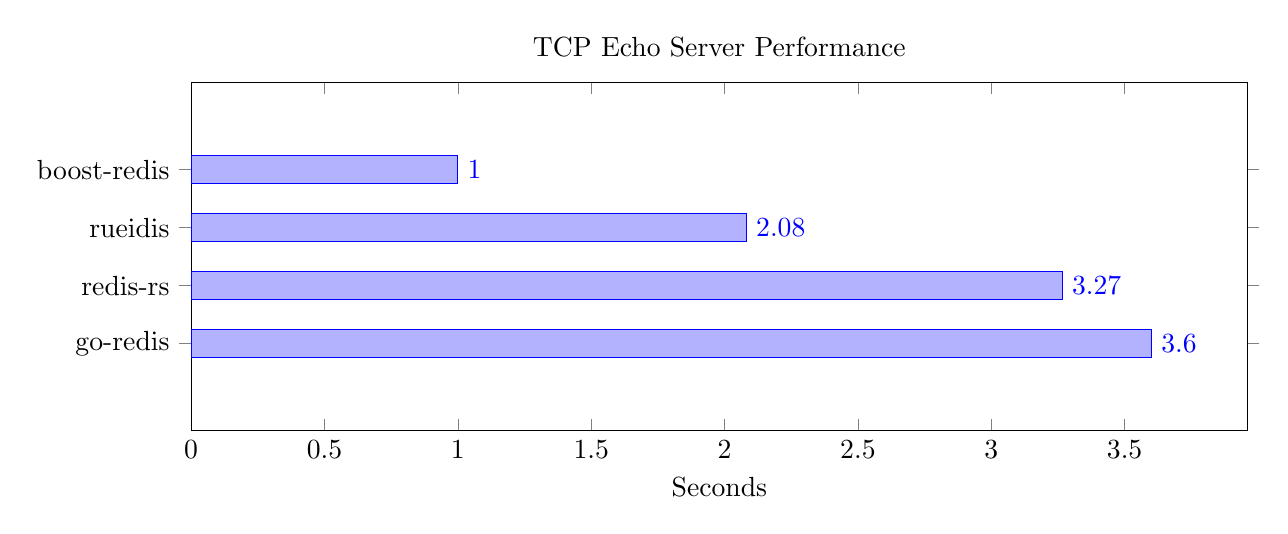
\begin{tikzpicture}[scale=1.0]
  \begin{axis}[
    y dir=reverse,
    %xbar stacked,
    xbar, xmin=0,
    %hide x axis,
    bar shift=0pt,
    width=15cm, height=6cm, enlarge y limits=0.5,
    title={TCP Echo Server Performance},
    xlabel={Seconds},
    symbolic y coords={boost-redis,rueidis,redis-rs,go-redis},
    ytick=data,
    %bar width=1cm,
    nodes near coords,
    nodes near coords align={horizontal},
    ]
    \addplot coordinates {
       (1.000,boost-redis)
       (2.082,rueidis)
       (3.266,redis-rs)
       (3.601,go-redis)
    };
  \end{axis}
\end{tikzpicture}
\endpgfgraphicnamed

\end{document}
